\documentclass{article}
\usepackage{graphicx}
\usepackage{authblk}


\begin{document}

\title{Eagle: Making multiple-locus association mapping on a genome-wide scale routine}
\author[1]{Andrew W. George}
\author[2]{Joshua Bowden}
\author[1]{Some other authors}

\affil[1]{Data61, CSIRO, Brisbane, Australia.}
\affil[2]{IM \&T, CSIRO, Brisbane, Australia.}

\maketitle


\begin{figure}
\caption{Memory usage (in Gigabytes) of Eagle and the other association mapping programs across 
the six simulation scenarios. The maximum amount of memory on the computer is 128 Gigabytes. 
The x-axis is on the log scale. GEMMA, a single-locus implementation, had the lowest memory usage. 
Of the multiple-locus implementations, Eagle had the lowest memory usage. Also, it 
was the only multiple-locus 
implementation able to produce results for data under  scenario 10000x1.5M. This is due to its ability 
to handle data larger than the available memory of a computer. FaST-LMM was run where all the snp data are used 
to estimate the relationship matrix (FaST-LMM$^{all}$)   and where genotype data from every five-hundredth snp are used to 
estimate the relationship matrix (FaST-LMM$^{few}$)}.
\begin{center}
\includegraphics[width=15cm, height=15cm]{mem.eps}
\end{center}
\end{figure}


\begin{table}
\caption{The median run times (in minutes) of Eagle and the other association mapping programs across the six simulation scenarios. The }
\begin{tabular}{llcccccc}
              &           &  \multicolumn{6}{c}{Simulation Scenarios} \\ \cline{3-8}
 Method & Name & 150x5K & 1500x50K & 350x400K & 2000x500K & 4000x1.5M & 10000x1.5M \\ \hline
  Multiple & Eagle 	&	   0.08  &   1.62   &  \bf{2.7}1  &   \bf{13.65}   & \bf{127.63}  &   699.55  \\
               & MLMM 	&	   0.15    &  2.91    & 19.04  &  143.01  &  870.84  &     \\
               & glmnet 	&	  0.11     & 3.95    & 14.06    & 74.03    &        &    \\
               & r2VIM 	&	   0.09    &  3.66    &  5.51    & 50.59    & 380.52  &   \\ 
               & bigRR 	&	    1.01   & 113.35   &  54.99   & 1030.61  &        &     \\
               & LMM-Lasso 	&     0.57  &   52.08 &    92.20  & 1031.85 &           &     \\ \\
Single     &  GEMMA 	&      0.02  &   5.02   &   6.17  &   84.83   & 723.33  & 4071.60 \\
               & FaST-LMM$^{few}$ 	&    \bf{0.01}   &  \bf{0.80}   &   7.07   &  20.16   & 193.90   & \bf{346.19} \\ 
               & FaST-LMM$^{all}$   	&   0.03   & 2.96  &    7.90   &  41.27  &            &   \\ \hline
\end{tabular}

\end{table}


\end{document}
